\section{Clase 11}
\subsection{Grupo de Galileo y sus cargas conservadas}
Consideremos la función de Lagrange 
\begin{equation}
  L=\frac{1}{2}\sum_i m_i\dot{x}^2_i+\sum_{i<j}V|x_i-x_j|
\end{equation}
es invariante bajo el grupo de Galileo. A saber,

\textbf{Traslaciones temporales:} $G_\t :t'=t+\t =f(t,\t )$. 

Siguiendo el procedimiento usual, $a_\n \leftrightarrow \t ,\, \n =1$ y $x_i\leftrightarrow t$. Luego
\begin{equation}
  u_{11}=1,\quad X_\n =\sum_i u_{i\n }\pdv{x_i}
\end{equation}
\begin{equation}
  X=\pdv{t}=H\implies H=\pdv{t}
\end{equation}

\textbf{Traslaciones espaciales:} $G_a :x'=x_i+a_i=f(x_{i},a_{i})$.
\begin{equation}
  u_{11}=1,\qquad X=\pdv{x_i}\implies P_i=\pdv{x}
\end{equation}

\textbf{Rotaciones temporales:} $G_R :x'=x_i+R_{i}^j x_j=f(x_{i},\th )$.

Anteriormente determinamos los generadores de $SO(3)$,
\begin{align}
  X_{12}&=x_1\pdv{x_2}-x_2\pdv{x_1} \quad \longrightarrow X_3\\
  X_{23}&=x_2\pdv{x_3}-x_3\pdv{x_2}\quad \longrightarrow X_1\\
  X_{31}&=x_3\pdv{x_1}-x_1\pdv{x_3}\quad \longrightarrow X_2
\end{align}
de manera que
\begin{equation}
  X_i=\epsilon_{ijk}x_j\pdv{x^k}\equiv J_i
\end{equation}

\textbf{Boosts de Galileo:} $G_v :x'=x_i+v_it=f(x_i,v_i)$.
\begin{equation}
  u_{11}=t,\qquad X_i=t\pdv{x^{i}},\qquad G_i=t\pdv{x^{i}}\equiv t P_i
\end{equation}

Así tenemos que los generadores del grupo de Galileo son $\{H,P_i,J_i,G_i\}$ donde
\begin{align}
  H&=\pdv{t}\\
  P_i&=\pdv{x^{i}}\\
  J_i&=\epsilon_{ijk}x_j\pdv{x^k}\\
  G_i&=t\pdv{x^{i}}
\end{align}

\subsection{Partícula libre en $3$-dimensiones}
Las ecuaciones de Newton son invariantes bajo el grupo de transformaciones de Galileo. Normalmente es aceptado que las transformaciones de Galileo son las simetrías más generales bajo la cual las ecuaciones de Newton permanecen invariantes en forma.

Sin embargo, notemos que la trayectoria de una partícula libre que parte desde $\vec{x}_0$ con velocidad $\vec{v}_0$ es igual a 
\begin{equation}\label{11.1}
  \vec{x}(t)=\vec{x}_0+\vec{v}_0t
\end{equation}
que relaciona las posiciones de la partícula. Escribiendo \eqref{11.1} en la forma
\begin{equation}\label{11.2}
  \frac{\vec{x}(t)}{t}=\frac{\vec{x}_0}{t}+\vec{v}_0
\end{equation}
Si llamamos $\tilde{\vec{x}}(t)=\vec{x}(t)/t$ y $\tilde{t}=1/t$, tenemos
\begin{equation}
  \tilde{\vec{x}}(t)=\vec{v}_0+\vec{x}_0\tilde{t}
\end{equation}
que relaciona velocidades. Notemos que existe una dualidad entre \eqref{11.1} y \eqref{11.2}.

En Ref. \cite{Jahn:2001qk} fue encontrado que el grupo de transformaciones más general que deja invariante la ecuación de Newton es un grupo de $12$ generadores ($12$ parámetros) constituido por
\begin{itemize}
	\item El grupo de Galileo de $10$ parámetros.
	\item El grupo de dilataciones de $1$ parámetro.
	\item El grupo de expansiones de $1$ parámetro.
\end{itemize}

 Los generadores de este grupo general son:
\begin{align*}
  H&=\pdv{t}\\
  P_i&=\pdv{q^{i}}\\
  J_i&=\epsilon_{ijk}q_j\pdv{q^k}\\
  G_i&=t\pdv{q^{i}}\\
  S&=2t\pdv{t}+q^{i}\pdv{q^{i}}\\
  C&=t^2\pdv{t}+tq^{i}\pdv{q^{i}}
\end{align*}
Este grupo es conocido como el \textit{grupo de Schrödinger} que también deja invariante la ecuación de Schrödinger (Ver Ref. \cite{Niederer:1972zz}).

\part{Electrodinámica y Relatividad}
\subsection{Transformaciones de Galileo y ecuaciones de Newton}
Consideremos dos SRI $K$ y $K'$. La relación entre las mediciones de ambos SRI está dado por
\begin{equation}
  x'=x-vt,\qquad y'=y,\qquad z'=z,\qquad t'=t
\end{equation}

\begin{figure}[h!]
	\centering
	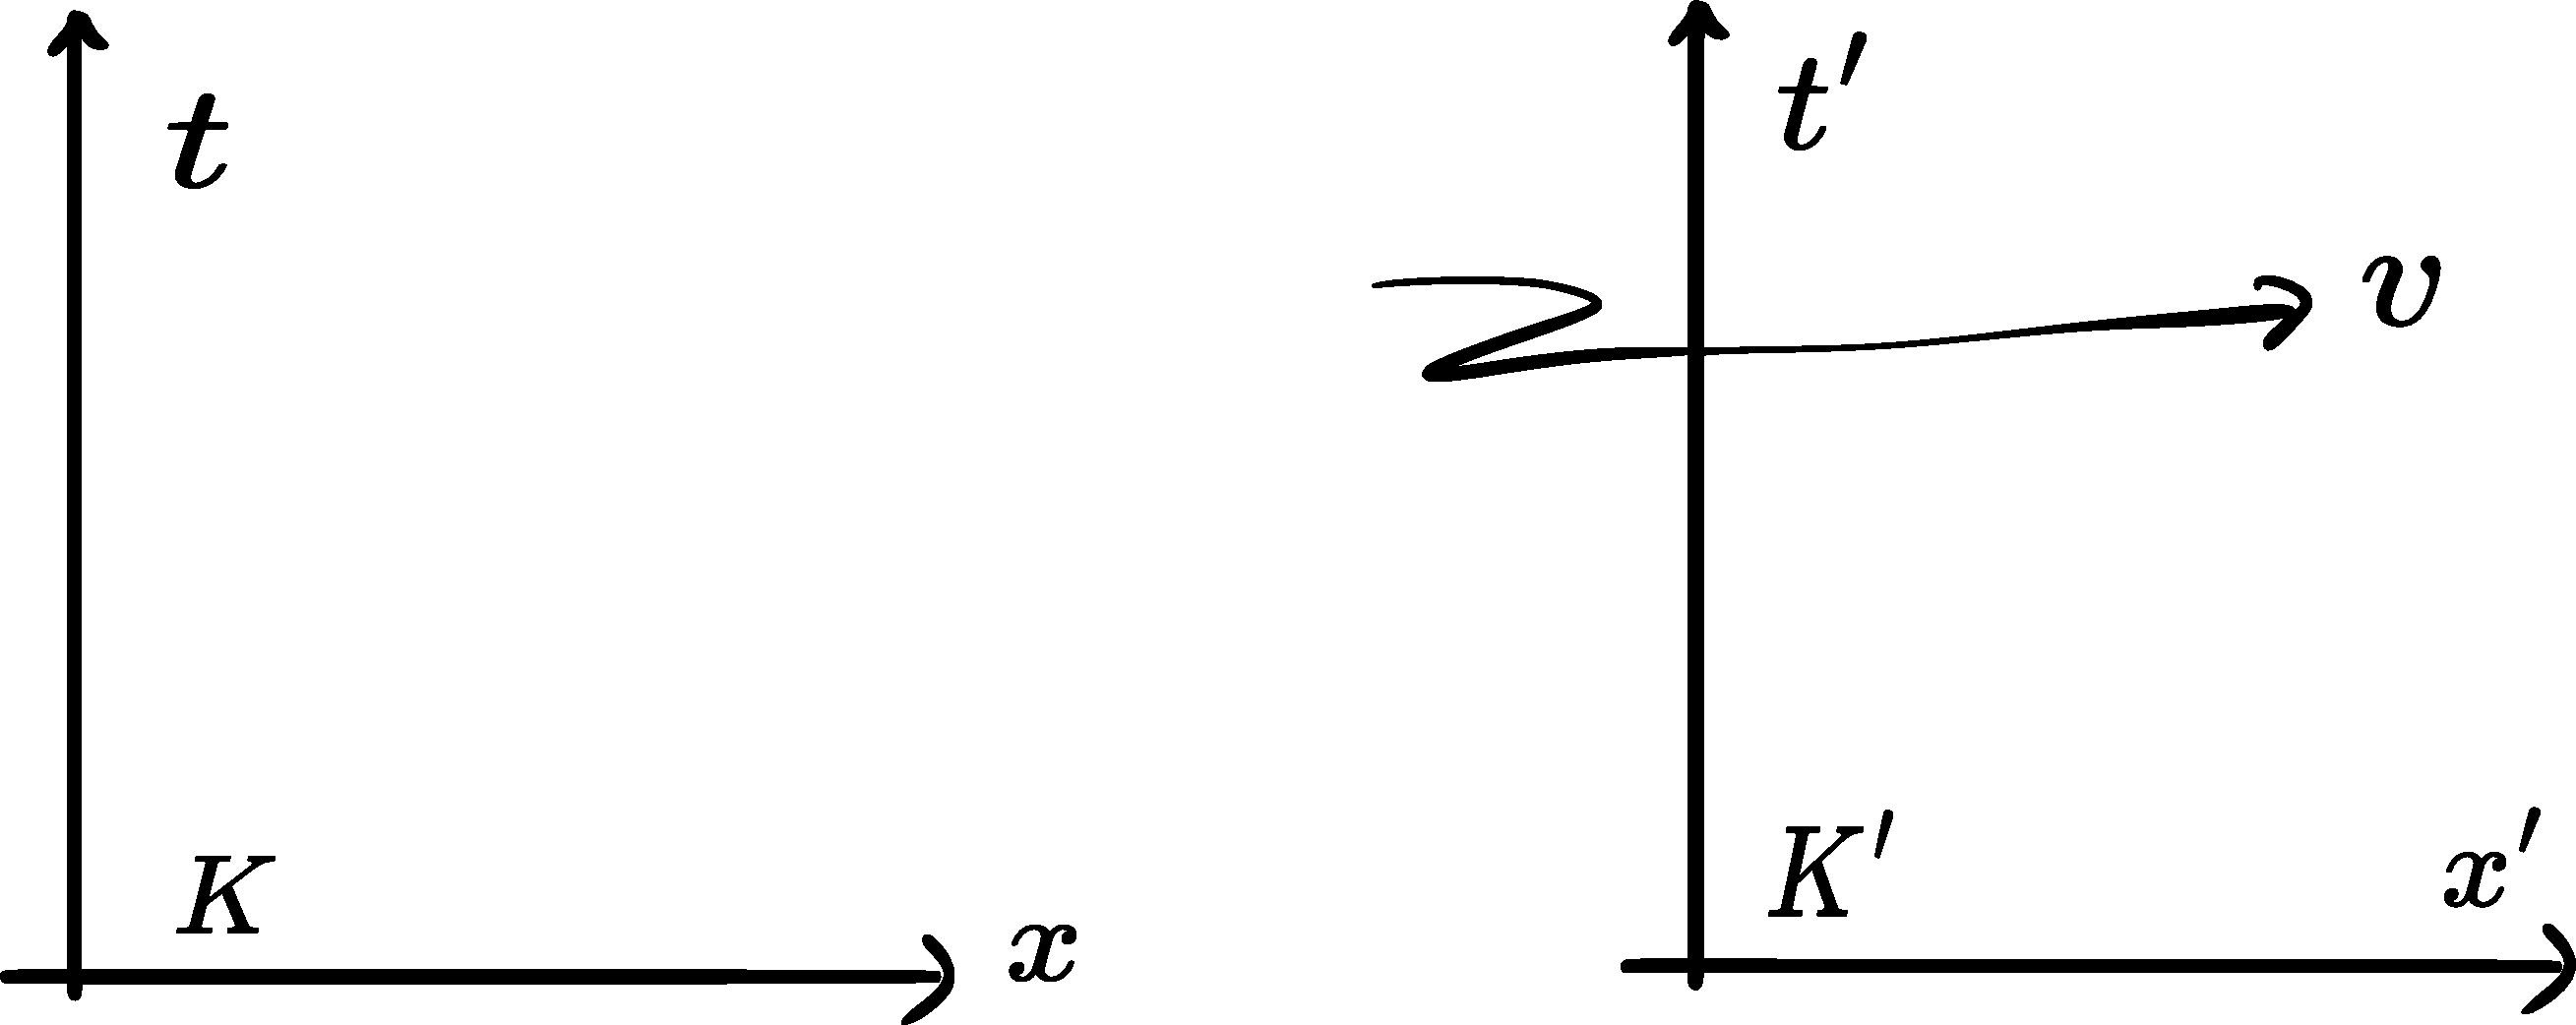
\includegraphics[scale=0.2]{fig/Galileo.pdf}
\end{figure}

La covariancia de las leyes de la física implican que las leyes de Newton en $K$ deben tener la misma forma en $K'$,
\begin{align}
  K&:\quad \vec{F}=m\vec{a}\\
  K'&:\quad \vec{F}'=m'\vec{a}'
\end{align}
Veamos si $F=ma$ es invariante bajo Galileo: \footnote{Por simplicidad consideremos una sóla dimensión.}
\begin{equation}
  x'=x-vt\implies \dv{x'}{t'}=\dv{x}{t}-v
\end{equation}
Definiendo la velocidad medida en $K$ con $V=\dv*{x}{t}$ y la velocidad medida en $K'$ con $V'=\dv*{x'}{t'}$ tenemos
\begin{equation}
  V'=V-v\implies \boxed{V'\neq V}
\end{equation}
es decir, la velocidad es una cantidad relativa.

\begin{equation}
  \dv{V'}{t'}=\dv{V}{t}-\dv{v}{t}
\end{equation}
pero $v$ es constante, luego
\begin{equation}
  \dv{V'}{t'}=\dv{V}{t}\implies \boxed{a'=a}
\end{equation}
es decir, la aceleración es una cantidad absoluta. Dado que por postulado la masa es una cantidad absoluta $m'=m$, se tiene
\begin{equation}
\boxed{  F'=F}
\end{equation}

 En este punto es natural hacerse la siguiente pregunta: ¿Son todas las leyes de la física invariante en forma? o ¿Son todas las leyes de la física invariantes en forma bajo Galileo?
 
 Las ecuaciones de Maxwell en el vacío vienen dadas por:
 \begin{align}
  &\nabla\cdot\vec{E}=0\label{11.11}\\
  &\nabla\cdot\vec{B}=0\label{11.12}\\
  &\nabla\times \vec{E}=-\pdv{\vec{B}}{t}\label{11.13}\\
  &\nabla\times \vec{B}=\m_0\ep_0\pdv{\vec{E}}{t}\label{11.14}
\end{align}
tomando el rotacional de \eqref{11.13} tenemos
\begin{align}
  \nabla\times \nabla \times\vec{E}&=-\nabla\times \pdv{\vec{B}}{t}=-\pdv{t}(\nabla\times\vec{B})\\
  &=-\pdv{t}\left(\m_0\ep_0\pdv{\vec{E}}{t}\right)\\
  &=-\m_0\ep_0\pdv[2]{\vec{E}}{t}
\end{align}
usando la identidad del cálculo vectorial, se tiene
\begin{align}
  \nabla(\cancelto{0}{\nabla\cdot\vec{E}})-\nabla^2\vec{E}=-\m_0\ep_0\pdv[2]{\vec{E}}{t}
\end{align}
\begin{equation}
  \implies \nabla^2\vec{E}-\m_0\ep_0\pdv[2]{\vec{E}}{t}=0
\end{equation}
Del mismo modo tenemos
\begin{equation}
  \nabla^2\vec{B}-\m_0\ep_0\pdv[2]{\vec{B}}{t}=0
\end{equation}
Cada componente $E_x,E_y,E_z,B_x,B_y,B_z$ satisface la ecuación
\begin{equation}\label{11.onda}
  \nabla^2\psi-\frac{1}{c^2}\pdv[2]{\psi}{t}=0,\qquad c^2=\frac{1}{\m_0\ep_0}
\end{equation}



\begin{ej}
	Probar que las ecuaciones de Maxwell no son invariantes bajo las transformaciones de Galileo, es decir, que las ecuaciones de Maxwell cambian de forma.
\end{ej}
\begin{sol}
	\begin{equation}
  x'=x-vt,\qquad y'=y,\qquad z'=z,\qquad t'=t
\end{equation}
esto implica que
\begin{equation}
  \pdv{x'}{x}=1,\qquad \pdv{x'}{t}=-v,\qquad \pdv{t'}{x}=0,\qquad \pdv{t'}{t}=1
\end{equation}
Luego,
\begin{equation}\label{11.trans}
\begin{split}
  \pdv{x}&=\pdv{x'}\pdv{x'}{x}+\pdv{t'}\pdv{t'}{x}=\pdv{x'}\\
  \pdv{t}&=\pdv{x'}\pdv{x'}{t}+\pdv{t'}\pdv{t'}{t}=\pdv{t'}-v\pdv{x'}
 \end{split}
\end{equation}
Las ecuaciones de Maxwell en una dimensión quedan
\begin{align}
  \nabla\cdot\vec{E}=0&\Longrightarrow \pdv{E_x}{x}=0\\
  \nabla\cdot\vec{B}=0&\Longrightarrow \pdv{B_x}{x}=0\\
  \nabla\times \vec{E}=-\pdv{\vec{B}}{t}&\Longrightarrow \pdv{E_z}{y}-\pdv{E_y}{z}=-\pdv{B_x}{t}\\
  \nabla\times \vec{B}=\m_0\ep_0\pdv{\vec{E}}{t}&\Longrightarrow \pdv{B_z}{y}-\pdv{B_y}{z}=\m_0\ep_0\pdv{E_x}{t}\\
\end{align}
Aplicando la transformación de Galileo, de \eqref{11.trans} se tiene
\begin{align}
  \pdv{E_x'}{x'}&=0\\
  \pdv{B_x'}{x'}&=0\\
  \pdv{E_z'}{y'}-\pdv{E_y'}{z'}&=-\pdv{B_x'}{t'}=-\left(\pdv{B_x'}{t'}-v\pdv{B_x'}{x'}\right)\\
  \pdv{B_z'}{y'}-\pdv{B_y'}{z'}&=\m_0\ep_0\pdv{E_x'}{t'}=\m_0\ep_0\left(\pdv{E_x'}{t'}-v\pdv{E_x'}{x'}\right)
\end{align}
Notar que estas dos últimas ecuaciones cambian en forma. Luego, bajo transformaciones de Galileo las ecuaciones de Maxwell cambian en forma.
\end{sol}

\begin{ej}
	Probar que la ecuación de la onda \eqref{11.onda} no es invariante bajo transformaciones de Galileo.
\end{ej}



